\documentclass{csbeamer}

\usepackage{dsfont}
\usepackage{amsmath}
\usepackage{amssymb}
\usepackage{listings}
\usepackage{algorithm}
\usepackage{algpseudocode}
\usepackage{tikz}
\usetikzlibrary{positioning, shapes, arrows, calc}

% Add custom color definitions for Deep RL (matching main file)
\definecolor{drlmain}{HTML}{6A1B9A}
\definecolor{drlaccent}{HTML}{FF6B35}
\definecolor{drllight}{HTML}{9C27B0}
\definecolor{drlsecondary}{HTML}{00897B}
\definecolor{drlpolicy}{HTML}{D32F2F}
\definecolor{drlvalue}{HTML}{1976D2}
\definecolor{drlactor}{HTML}{E91E63}
\definecolor{drlcritic}{HTML}{3F51B5}
\definecolor{drlgradient}{HTML}{FF9800}
\definecolor{drladvantage}{HTML}{4CAF50}
\definecolor{drlneural}{HTML}{7B1FA2}

\university{St. Francis Xavier University}
\department{Department of Computer Science}
\course{CSCI-531 - Reinforcement Learning}
\courseshort{CSCI-531 - RL}
\term{Fall 2025}
\author{Dr. Jean-Alexis Delamer}

\title{Proximal Policy Optimization (PPO)}

\begin{document}

\maketitle

\section{Introduction}

\subsection{Motivation}

\begin{frame}
    \frametitle{Quick Recap: What We Know So Far}

    \begin{block}<1->{Policy Gradient Methods (REINFORCE, A2C)}
        \begin{itemize}
            \item<2-> We directly optimize the policy $\pi_\theta(a|s)$ to maximize rewards
            \item<3-> Update rule: Increase probability of good actions, decrease bad ones
            \item<4-> \textcolor{drladvantage}{\textbf{Works well}}: Handles continuous actions, stochastic policies
        \end{itemize}
    \end{block}

    \begin{block}<5->{But There's a Critical Problem...}
        \begin{itemize}
            \item<6-> \textcolor{drlaccent}{\textbf{Sample efficiency}}: Need many environment interactions
            \item<7-> \textcolor{drlaccent}{\textbf{Sensitivity to step size}}: Hard to tune learning rate
            \item<8-> \textcolor{drlaccent}{\textbf{Stability}}: Training can suddenly collapse!
        \end{itemize}
    \end{block}

    \begin{block}<9->{Today's Goal}
        Understand why this happens and \textcolor{drlmain}{\textbf{how PPO fixes it}}.
    \end{block}
\end{frame}

\begin{frame}
    \frametitle{A Concrete Example: CartPole}

    \begin{block}<1->{Imagine Training CartPole with A2C}
        You've been training for a while, and your policy is doing well
    \end{block}

    \begin{block}<2->{You collect data and compute gradients...}
        \begin{itemize}
            \item<3-> Advantage says: "Right was a really good action! Advantage = +5.0"
            \item<4-> Standard policy gradient says: "Increase probability of right!"
        \end{itemize}
    \end{block}

    \begin{block}<5->{After One Big Update:}
        \begin{itemize}
            \item<6-> New policy: Move left: $0.01$, Move right: $\textcolor{drlaccent}{0.99}$
            \item<7-> \textcolor{drlaccent}{\textbf{Too extreme!}} Policy became nearly deterministic
            \item<8-> \textcolor{drlaccent}{\textbf{Result:}} Can't explore anymore, training collapses!
        \end{itemize}
    \end{block}
\end{frame}

\begin{frame}
    \frametitle{Visualizing the Step Size Problem}

    \begin{center}
        \begin{tikzpicture}[scale=0.9]
            % Performance curve
            \draw[->] (0,0) -- (9,0) node[right] {Policy Parameters $\theta$};
            \draw[->] (0,0) -- (0,5) node[above] {Performance $J(\theta)$};

            % Draw a curved performance surface
            \draw[drlmain, thick] plot[smooth, domain=0:8]
                (\x, {2 + 1.5*sin((\x)*60) + 0.3*(\x-4)*(\x-4)/10});

            % Current policy
            \fill[drlpolicy] (0.4,3) circle (3pt) node[above left] {$\pi_{\theta_{\text{old}}}$};

            % Small step (good)
            \only<2->{
                \draw[->, drladvantage, very thick] (0.4,3) -- (1.2,3.65);
                \fill[drladvantage] (1.2,3.65) circle (3pt) node[above] {\small Good step};
            }

            % Large step (bad)
            \only<3->{
                \draw[->, drlaccent, very thick] (0.4,3) -- (5.6,1.5);
                \fill[drlaccent] (5.6,1.5) circle (3pt) node[below right] {\small \textbf{Policy collapse!}};
            }

            % Highlight regions
            \only<4->{
                \draw[drladvantage, dashed, thick] (0.4,3) circle (1.2cm);
                \node[drladvantage] at (0.5,4.5) {\small Trust region};
            }
        \end{tikzpicture}
    \end{center}

    \begin{block}<4->{Key Insight}
        We need to \textcolor{drlmain}{\textbf{limit how much the policy can change}} in each update!
    \end{block}
\end{frame}

\begin{frame}
    \frametitle{Evolution of Policy Optimization}

    \begin{block}<1->{The Journey to PPO}
        \begin{enumerate}
            \item<2-> \textcolor{gray}{\textbf{REINFORCE (1992)}}: Basic policy gradient, high variance
            \item<3-> \textcolor{gray}{\textbf{A2C/A3C (2016)}}: Actor-critic, better but still unstable
            \item<4-> \textcolor{drlsecondary}{\textbf{TRPO (2015)}}: Trust Region Policy Optimization
                \begin{itemize}
                    \item<5-> Constrains policy updates using KL divergence
                    \item<6-> Guarantees monotonic improvement
                    \item<7-> \textcolor{drlaccent}{\textbf{Problem}}: Complex, computationally expensive
                \end{itemize}
            \item<8-> \textcolor{drlmain}{\textbf{PPO (2017)}}: Simplified TRPO
                \begin{itemize}
                    \item<9-> \textcolor{drladvantage}{Simpler to implement}
                    \item<10-> \textcolor{drladvantage}{Better sample efficiency}
                    \item<11-> \textcolor{drladvantage}{State-of-the-art performance}
                \end{itemize}
        \end{enumerate}
    \end{block}
\end{frame}

\subsection{PPO Overview}

\begin{frame}
    \frametitle{What is PPO?}

    \begin{block}<1->{Proximal Policy Optimization}
        An actor-critic algorithm that constrains policy updates to stay \textcolor{drlmain}{\textbf{close}} to the old policy
    \end{block}

    \begin{block}<2->{The Core Innovation (in plain English)}
        \begin{itemize}
            \item<3-> \textbf{A2C says:} "If action was good, increase its probability as much as the gradient says"
            \item<4-> \textbf{PPO says:} "If action was good, increase its probability, but \textcolor{drlmain}{NOT TOO MUCH!}"
        \end{itemize}
    \end{block}

    \begin{block}<5->{Four Key Ideas}
        \begin{enumerate}
            \item<6-> \textcolor{drlpolicy}{\textbf{Clipped objective}}: The "not too much" mechanism
            \item<7-> \textcolor{drlsecondary}{\textbf{Multiple epochs}}: Reuse same data multiple times
            \item<8-> \textcolor{drlcritic}{\textbf{Value function}}: Same critic as A2C
            \item<9-> \textcolor{drladvantage}{\textbf{Simple}}: Easier than older methods (TRPO)
        \end{enumerate}
    \end{block}

    \begin{block}<7->{Why "Proximal"?}
        \textit{Proximal} means "nearby" -- we keep the new policy \textcolor{drlmain}{\textbf{close}} to the old one!
    \end{block}
\end{frame}

\section{PPO Theory}

\subsection{The Probability Ratio}

\begin{frame}
    \frametitle{Understanding the Ratio Trick}

    \begin{block}<1->{Standard Policy Gradient Objective}
        \begin{equation*}
            L^{\text{PG}}(\theta) = \mathbb{E}_t \left[ A_t \log \pi_\theta(a_t|s_t) \right]
        \end{equation*}
    \end{block}

    \begin{block}<2->{Rewrite Using Probability Ratio}
        Define the ratio:
        \begin{equation*}
            r_t(\theta) = \frac{\pi_\theta(a_t|s_t)}{\pi_{\theta_{\text{old}}}(a_t|s_t)}
        \end{equation*}
        \vspace{-0.3cm}
        \begin{itemize}
            \item<3-> $r_t(\theta_{\text{old}}) = 1$ (identical policies)
            \item<4-> $r_t(\theta) > 1$ means action is \textcolor{drladvantage}{more likely} under new policy
            \item<5-> $r_t(\theta) < 1$ means action is \textcolor{drlaccent}{less likely} under new policy
        \end{itemize}
    \end{block}
\end{frame}

\begin{frame}
    \frametitle{Understanding the Ratio Trick}

    \begin{block}{Standard Policy Gradient Objective}
        \begin{equation*}
            L^{\text{PG}}(\theta) = \mathbb{E}_t \left[ A_t \log \pi_\theta(a_t|s_t) \right]
        \end{equation*}
    \end{block}

    \begin{block}{Rewrite Using Probability Ratio}
        Define the ratio:
        \begin{equation*}
            r_t(\theta) = \frac{\pi_\theta(a_t|s_t)}{\pi_{\theta_{\text{old}}}(a_t|s_t)}
        \end{equation*}
    \end{block}

    \begin{block}{Equivalent Objective (for importance sampling)}
        \begin{equation*}
            L^{\text{CPI}}(\theta) = \mathbb{E}_t \left[ r_t(\theta) A_t \right]
        \end{equation*}
        \textcolor{gray}{\small CPI = Conservative Policy Iteration}
    \end{block}
\end{frame}

\begin{frame}
    \frametitle{The Problem with Unconstrained Updates}

    \begin{block}<1->{The CPI Objective}
        \begin{equation*}
            L^{\text{CPI}}(\theta) = \mathbb{E}_t \left[ \frac{\pi_\theta(a_t|s_t)}{\pi_{\theta_{\text{old}}}(a_t|s_t)} A_t \right]
        \end{equation*}
    \end{block}

    \begin{block}<2->{What Could Go Wrong?}
        \begin{itemize}
            \item<3-> If $A_t > 0$ (good action), optimizer tries to make $r_t(\theta) \to \infty$
            \item<4-> If $A_t < 0$ (bad action), optimizer tries to make $r_t(\theta) \to 0$
            \item<5-> \textcolor{drlaccent}{\textbf{Result}}: Policy changes too drastically!
        \end{itemize}
    \end{block}

    \begin{block}<6->{The Solution}
        \textcolor{drlmain}{\textbf{Clip the ratio}} to prevent extreme updates!
    \end{block}
\end{frame}

\subsection{The Clipped Objective}

\begin{frame}
    \frametitle{PPO-Clip: The Main Innovation}

    \begin{block}<1->{PPO Clipped Objective}
        \begin{equation*}
            L^{\text{CLIP}}(\theta) = \mathbb{E}_t \left[ \min\left( r_t(\theta) A_t, \text{clip}(r_t(\theta), 1-\epsilon, 1+\epsilon) A_t \right) \right]
        \end{equation*}
        where $\epsilon$ is a hyperparameter (typically $0.1$ or $0.2$)
    \end{block}

    \begin{block}<2->{Breaking It Down (Step-by-Step)}
        \begin{enumerate}
            \item<3-> \textcolor{drlmain}{\textbf{clip}$(r, 1-\epsilon, 1+\epsilon)$}: Force ratio into range [0.8, 1.2]
                \begin{itemize}
                    \item If $r = 1.5$, clipped value = 1.2
                    \item If $r = 0.5$, clipped value = 0.8
                    \item If $r = 1.1$, clipped value = 1.1 (no change)
                \end{itemize}
            \item<4-> Compute two objectives:
                \begin{itemize}
                    \item Unclipped: $r_t \cdot A_t$
                    \item Clipped: $\text{clip}(r_t, 0.8, 1.2) \cdot A_t$
                \end{itemize}
            \item<5-> \textcolor{drlmain}{\textbf{min}}: Take the \textbf{pessimistic} (lower) of the two
        \end{enumerate}
    \end{block}
\end{frame}

\begin{frame}
    \frametitle{PPO-Clip: The Main Innovation}

    \begin{block}{PPO Clipped Objective}
        \begin{equation*}
            L^{\text{CLIP}}(\theta) = \mathbb{E}_t \left[ \min\left( r_t(\theta) A_t, \text{clip}(r_t(\theta), 1-\epsilon, 1+\epsilon) A_t \right) \right]
        \end{equation*}
        where $\epsilon$ is a hyperparameter (typically $0.1$ or $0.2$)
    \end{block}

    \begin{block}{Effect}
        Policy can't change more than $\pm \epsilon$ per update!
    \end{block}
\end{frame}

\begin{frame}
    \frametitle{Numerical Example: How Clipping Works}

    \begin{itemize}
        \item Action had \textcolor{drladvantage}{positive advantage}: $A_t = +2.0$
        \item Clip range: $\epsilon = 0.2$ (so ratios allowed in [0.8, 1.2])
    \end{itemize}

    \begin{block}<2->{Different Ratio Scenarios}
        \small
        \begin{tabular}{ccccc}
            \textbf{Ratio} & \textbf{Unclipped} & \textbf{Clipped} & \textbf{min} & \textbf{Result} \\
            $r_t$ & $r \cdot A$ & $\text{clip}(r) \cdot A$ & & \\
            \hline
            0.6 & $0.6 \times 2 = 1.2$ & $0.8 \times 2 = 1.6$ & 1.2 & \textcolor{gray}{Use unclipped} \\
            1.0 & $1.0 \times 2 = 2.0$ & $1.0 \times 2 = 2.0$ & 2.0 & \textcolor{drladvantage}{No clipping} \\
            1.5 & $1.5 \times 2 = 3.0$ & $1.2 \times 2 = 2.4$ & 2.4 & \textcolor{drlaccent}{Clipped!} \\
            2.0 & $2.0 \times 2 = 4.0$ & $1.2 \times 2 = 2.4$ & 2.4 & \textcolor{drlaccent}{Clipped!} \\
        \end{tabular}
    \end{block}

    \begin{block}<3->{Key Insight}
        \begin{itemize}
            \item<4-> Once $r > 1.2$, further increases \textcolor{drlmain}{\textbf{don't help}} the objective
            \item<5-> No incentive to make the action even more likely!
            \item<6-> This is the \textcolor{drlmain}{\textbf{"trust region"}} in action
        \end{itemize}
    \end{block}
\end{frame}

\begin{frame}
    \frametitle{Visualizing the Clipped Objective (Positive Advantage)}

    \begin{center}
        \begin{tikzpicture}[scale=0.9]
            % Axes
            \draw[->] (0,0) -- (7,0) node[right] {$r_t(\theta)$};
            \draw[->] (0,0) -- (0,5) node[above] {Objective};

            % Mark key points
            \draw[dashed, gray] (1,0) -- (1,2) node[below left, yshift=-0.6cm] {$1-\epsilon$};
            \draw[dashed, gray] (3.5,0) -- (3.5,3) node[below, yshift=-0.2cm] {$1$};
            \draw[dashed, gray] (6,0) -- (6,4) node[below right, yshift=-0.6cm] {$1+\epsilon$};

            % Unclipped (linear)
            \only<2->{
                \draw[drlaccent, very thick, dashed] (0,1.6) -- (7,4.4);
                \node[drlaccent] at (6.5,5) {\small Unclipped};
            }

            % Clipped
            \only<3->{
                \draw[drlmain, very thick] (0,1.6) -- (6,4);
                \draw[drlmain, very thick] (6,4) -- (7,4);
                \node[drlmain] at (1.5,3) {\small PPO-Clip};
            }

            % Annotations
            \only<4->{
                \node[anchor=west, text width=2.5cm, drladvantage] at (7.5,3)
                    {No incentive to increase $r$ beyond $1+\epsilon$};
                \draw[->, drladvantage, thick] (7.5,2.8) -- (6,4);
            }

            \node[anchor=north] at (3.5,-0.5) {\textcolor{drladvantage}{Case: $A_t > 0$ (good action)}};
        \end{tikzpicture}
    \end{center}
\end{frame}

\begin{frame}
    \frametitle{Visualizing the Clipped Objective (Negative Advantage)}

    \begin{center}
        \begin{tikzpicture}[scale=0.9]
            % Axes
            \draw[->] (0,0) -- (7,0) node[right] {$r_t(\theta)$};
            \draw[->] (0,0) -- (0,-5) node[below] {Objective};

            % Mark key points
            \draw[dashed, gray] (1,0) -- (1,-2) node[above left, yshift=0.6cm] {$1-\epsilon$};
            \draw[dashed, gray] (3.5,0) -- (3.5,-3) node[above, yshift=0.2cm] {$1$};
            \draw[dashed, gray] (6,0) -- (6,-4) node[above right, yshift=0.6cm] {$1+\epsilon$};

            % Unclipped (linear, negative)
            \only<2->{
                \draw[drlaccent, very thick, dashed] (0,-1.6) -- (7,-4.4);
                \node[drlaccent] at (6.5,-5) {\small Unclipped};
            }

            % Clipped
            \only<3->{
                \draw[drlmain, very thick] (0,-2) -- (1,-2);
                \draw[drlmain, very thick] (1,-2) -- (7,-4.4);
                \node[drlmain] at (1.5,-3) {\small PPO-Clip};
            }

            % Annotations
            \only<4->{
                \node[anchor=west, text width=2.5cm, drladvantage] at (7.5,-1)
                    {No incentive to decrease $r$ beyond $1-\epsilon$};
                \draw[->, drladvantage, thick] (7.5,-1.2) -- (1.1,-2);
            }

            \node[anchor=south] at (3.5,0.5) {\small \textcolor{drlaccent}{Case: $A_t < 0$ (bad action)}};
        \end{tikzpicture}
    \end{center}
\end{frame}

\begin{frame}
    \frametitle{Understanding Both Cases}

    \begin{block}<1->{Case 1: Positive Advantage ($A_t > 0$)}
        \begin{itemize}
            \item<2-> Want to \textcolor{drladvantage}{increase} probability of action
            \item<3-> But only up to $(1+\epsilon) \pi_{\theta_{\text{old}}}(a_t|s_t)$
            \item<4-> \textcolor{drlmain}{Clip prevents over-optimism}
        \end{itemize}
    \end{block}

    \begin{block}<6->{Case 2: Negative Advantage ($A_t < 0$)}
        \begin{itemize}
            \item<5-> Want to \textcolor{drlaccent}{decrease} probability of action
            \item<6-> But only down to $(1-\epsilon) \pi_{\theta_{\text{old}}}(a_t|s_t)$
            \item<7-> \textcolor{drlmain}{Clip prevents over-correction}
        \end{itemize}
    \end{block}

    \begin{block}<8->{Result}
        Policy changes are \textcolor{drlmain}{\textbf{bounded}} and \textcolor{drladvantage}{\textbf{stable}}!
    \end{block}
\end{frame}

\subsection{Complete PPO Objective}

\begin{frame}
    \frametitle{The Full PPO Loss Function}

    \begin{block}<1->{Three Components}
        \begin{equation*}
            L^{\text{PPO}}(\theta) = L^{\text{CLIP}}(\theta) - c_1 L^{\text{VF}}(\theta) + c_2 H(\pi_\theta)
        \end{equation*}
    \end{block}

    \begin{block}<2->{Breaking It Down}
        \begin{enumerate}
            \item<3-> \textcolor{drlactor}{\textbf{Policy Loss}} $L^{\text{CLIP}}(\theta)$: $\mathbb{E}_t \left[ \min\left( r_t(\theta) A_t, \text{clip}(r_t(\theta), 1-\epsilon, 1+\epsilon) A_t \right) \right]$

            \item<4-> \textcolor{drlcritic}{\textbf{Value Function Loss}} $L^{\text{VF}}(\theta)$: $\mathbb{E}_t \left[ \left( V_\theta(s_t) - V_t^{\text{target}} \right)^2 \right]$

            \item<5-> \textcolor{drladvantage}{\textbf{Entropy Bonus}} $H(\pi_\theta)$: $\mathbb{E}_t \left[ -\sum_a \pi_\theta(a|s_t) \log \pi_\theta(a|s_t) \right]$

        \end{enumerate}
    \end{block}
\end{frame}

\begin{frame}
    \frametitle{Understanding Each Component}

    \begin{block}<1->{1. Policy Loss (Clipped Objective)}
        \begin{itemize}
            \item Updates the policy to increase good actions, decrease bad actions
            \item \textcolor{drlmain}{Clipping} ensures stable updates
        \end{itemize}
    \end{block}

    \begin{block}<2->{2. Value Function Loss}
        \begin{itemize}
            \item Trains the critic to predict returns accurately
            \item Used to compute advantages: $A_t = r_t + \gamma V(s_{t+1}) - V(s_t)$
        \end{itemize}
    \end{block}

    \begin{block}<3->{3. Entropy Bonus}
        \begin{itemize}
            \item Encourages exploration by penalizing deterministic policies
            \item Higher entropy $\rightarrow$ more random policy
        \end{itemize}
    \end{block}
\end{frame}

\section{PPO Algorithm}

\subsection{The PPO Algorithm}

\begin{frame}[fragile]
    \begin{algorithm}[H]
        \caption{Proximal Policy Optimization (PPO-Clip)}
        \begin{algorithmic}[1]
            \State Initialize policy network $\pi_\theta$ and value network $V_\phi$
            \For{iteration $= 1, 2, \ldots$}
                \For{actor $= 1, \ldots, N$} \textcolor{drlsecondary}{\textbf{// Collect trajectories}}
                    \State Run policy $\pi_{\theta_{\text{old}}}$ for $T$ timesteps
                    \State Collect $(s_t, a_t, r_t)$ and compute advantages $A_t$
                \EndFor
                \For{epoch $= 1, \ldots, K$} \textcolor{drlsecondary}{\textbf{// Optimize surrogate objective}}
                    \For{minibatch in trajectories}
                        \State Compute ratio: $r_t = \frac{\pi_\theta(a_t|s_t)}{\pi_{\theta_{\text{old}}}(a_t|s_t)}$
                        \State Compute clipped objective: $L^{\text{CLIP}}(\theta)$
                        \State Update $\theta$ by gradient ascent on $L^{\text{CLIP}}$
                        \State Update $\phi$ by gradient descent on value loss
                    \EndFor
                \EndFor
                \State $\theta_{\text{old}} \leftarrow \theta$
            \EndFor
        \end{algorithmic}
    \end{algorithm}
\end{frame}

\subsection{Key Differences from A2C}

\begin{frame}
    \frametitle{PPO vs A2C: Side-by-Side Comparison}

    \begin{center}
        \small
        \begin{tabular}{|l|p{3.5cm}|p{3.5cm}|}
            \hline
            \textbf{Feature} & \textbf{A2C} & \textbf{PPO} \\
            \hline
            \hline
            \textbf{Policy update} & Direct gradient ascent & Clipped ratio objective \\
            \hline
            \textbf{Data reuse} & \textcolor{drlaccent}{Each batch used once} & \textcolor{drladvantage}{Reuse for K epochs} \\
            \hline
            \textbf{Sample efficiency} & Moderate & \textcolor{drladvantage}{Better (K times)} \\
            \hline
            \textbf{Stability} & \textcolor{drlaccent}{Can be unstable} & \textcolor{drladvantage}{Very stable} \\
            \hline
            \textbf{Step size control} & Learning rate only & \textcolor{drladvantage}{Clipping + LR} \\
            \hline
            \textbf{Implementation} & \textcolor{drladvantage}{Simpler} & Moderate \\
            \hline
            \textbf{Time per update} & \textcolor{drladvantage}{Faster} & Slower (K epochs) \\
            \hline
            \textbf{Total training time} & Longer & \textcolor{drladvantage}{Often shorter!} \\
            \hline
        \end{tabular}
    \end{center}

    \begin{block}<2->{The Trade-off}
        PPO does \textcolor{drlaccent}{more computation per batch} but needs \textcolor{drladvantage}{fewer batches overall}
    \end{block}
\end{frame}

\begin{frame}
    \frametitle{Visual Comparison: Training Process}

    \begin{columns}
        \begin{column}{0.48\textwidth}
            \begin{block}<1->{A2C}
                \begin{enumerate}
                    \item<2-> Collect batch (e.g., 2048 steps)
                    \item<3-> Compute advantages
                    \item<4-> \textcolor{drlmain}{Update once}
                    \item<5-> \textcolor{drlaccent}{Throw away data}
                    \item<6-> Repeat: Collect new batch
                \end{enumerate}
                \vspace{0.3cm}
                \only<7->{\textcolor{drlaccent}{\textbf{Result}}: Need many batches}
            \end{block}
        \end{column}

        \begin{column}{0.48\textwidth}
            \begin{block}<1->{PPO}
                \begin{enumerate}
                    \item<2-> Collect batch (e.g., 2048 steps)
                    \item<3-> Compute advantages
                    \item<4-> \textcolor{drladvantage}{Update 10 times}
                    \item<5-> \textcolor{drladvantage}{(reuse same data)}
                    \item<6-> Then: Collect new batch
                \end{enumerate}
                \vspace{0.3cm}
                \only<7->{\textcolor{drladvantage}{\textbf{Result}}: Fewer batches needed}
            \end{block}
        \end{column}
    \end{columns}

    \begin{block}<8->{Why Can PPO Reuse Data?}
        \begin{itemize}
            \item<9-> Clipping ensures policy doesn't change too much
            \item<10-> After K epochs, policy has drifted from old policy
            \item<11-> Time to collect fresh data!
        \end{itemize}
    \end{block}
\end{frame}

\begin{frame}
    \frametitle{The Multiple Epochs Trick}

    \begin{block}<1->{Why Can PPO Reuse Data?}
        \begin{itemize}
            \item<2-> A2C is strictly on-policy: data from $\pi_{\theta_{\text{old}}}$ only valid for one update
            \item<3-> PPO uses \textcolor{drlmain}{importance sampling} with the ratio $r_t(\theta)$
            \item<4-> \textcolor{drladvantage}{Clipping} ensures we don't stray too far from $\pi_{\theta_{\text{old}}}$
        \end{itemize}
    \end{block}

    \begin{block}<5->{The Process}
        \begin{enumerate}
            \item<6-> Collect batch of trajectories with $\pi_{\theta_{\text{old}}}$
            \item<7-> Perform \textcolor{drlmain}{$K$ epochs} of minibatch updates (typically $K=3$ to $10$)
            \item<8-> Each minibatch update uses the same data but updated policy
            \item<9-> After $K$ epochs, collect new data and repeat
        \end{enumerate}
    \end{block}

    \begin{block}<10->{Result}
        \textcolor{drladvantage}{$K \times$ better sample efficiency!}
    \end{block}
\end{frame}

\section{PPO Implementation}

\subsection{Network Architecture}

\begin{frame}[fragile]
    \frametitle{PPO Network (Same as A2C)}

    \begin{block}<1->{Shared Network with Two Heads}
        \begin{lstlisting}[language=Python, basicstyle=\tiny\ttfamily, keywordstyle=\color{drlmain}, commentstyle=\color{gray}, stringstyle=\color{drlsecondary}]
class PPONetwork(nn.Module):
    def __init__(self, obs_dim, action_dim, hidden_dim=64):
        super().__init__()

        # Shared feature extractor
        self.shared = nn.Sequential(
            nn.Linear(obs_dim, hidden_dim),
            nn.Tanh(),
            nn.Linear(hidden_dim, hidden_dim),
            nn.Tanh()
        )

        # Policy head (actor)
        self.policy_head = nn.Linear(hidden_dim, action_dim)

        # Value head (critic)
        self.value_head = nn.Linear(hidden_dim, 1)

    def forward(self, state):
        features = self.shared(state)
        logits = self.policy_head(features)
        value = self.value_head(features)
        return logits, value
        \end{lstlisting}
    \end{block}
\end{frame}

\subsection{Computing the Clipped Loss}

\begin{frame}[fragile]
    \frametitle{Computing the PPO Clipped Objective}

    \begin{block}<1->{Step 1: Compute Old and New Probabilities}
        \begin{lstlisting}[language=Python, basicstyle=\tiny\ttfamily, keywordstyle=\color{drlmain}, commentstyle=\color{gray}, stringstyle=\color{drlsecondary}]
import torch.distributions as dist

# Get new policy distribution
logits, values = network(states)
new_policy = dist.Categorical(logits=logits)
new_log_probs = new_policy.log_prob(actions)

# Old log probs were stored during trajectory collection
old_log_probs = stored_log_probs  # from buffer

# Compute ratio
ratio = torch.exp(new_log_probs - old_log_probs)
# Equivalent to: ratio = new_probs / old_probs
        \end{lstlisting}
    \end{block}

    \begin{block}<2->{Why Log Space?}
        \begin{itemize}
            \item<3-> More numerically stable
            \item<4-> $\exp(\log p_{\text{new}} - \log p_{\text{old}}) = \frac{p_{\text{new}}}{p_{\text{old}}}$
        \end{itemize}
    \end{block}
\end{frame}

\begin{frame}[fragile]
    \frametitle{Computing the Clipped Loss (cont.)}

    \begin{block}<1->{Step 2: Compute Clipped Objective}
        \begin{lstlisting}[language=Python, basicstyle=\tiny\ttfamily, keywordstyle=\color{drlmain}, commentstyle=\color{gray}, stringstyle=\color{drlsecondary}]
# Hyperparameter
epsilon = 0.2

# Compute surrogate losses
surr1 = ratio * advantages
surr2 = torch.clamp(ratio, 1 - epsilon, 1 + epsilon) * advantages

# Take minimum (pessimistic bound)
policy_loss = -torch.min(surr1, surr2).mean()
        \end{lstlisting}
    \end{block}

    \begin{block}<2->{Breaking It Down}
        \begin{itemize}
            \item<3-> \texttt{surr1}: Unclipped objective $r_t(\theta) \cdot A_t$
            \item<4-> \texttt{surr2}: Clipped version with $r_t \in [1-\epsilon, 1+\epsilon]$
            \item<5-> \texttt{torch.min}: Takes element-wise minimum (pessimistic)
            \item<6-> Negative sign: Convert maximization to minimization for optimizer
        \end{itemize}
    \end{block}
\end{frame}

\begin{frame}[fragile]
    \frametitle{Value Loss and Entropy}

    \begin{block}<1->{Value Function Loss}
        \begin{lstlisting}[language=Python, basicstyle=\tiny\ttfamily, keywordstyle=\color{drlmain}, commentstyle=\color{gray}, stringstyle=\color{drlsecondary}]
# Compute value loss (MSE)
value_loss = ((returns - values) ** 2).mean()
        \end{lstlisting}
    \end{block}

    \begin{block}<2->{Entropy Bonus}
        \begin{lstlisting}[language=Python, basicstyle=\tiny\ttfamily, keywordstyle=\color{drlmain}, commentstyle=\color{gray}, stringstyle=\color{drlsecondary}]
# Compute entropy
entropy = new_policy.entropy().mean()
        \end{lstlisting}
    \end{block}

    \begin{block}<3->{Total Loss}
        \begin{lstlisting}[language=Python, basicstyle=\tiny\ttfamily, keywordstyle=\color{drlmain}, commentstyle=\color{gray}, stringstyle=\color{drlsecondary}]
# Combine all losses
value_coef = 0.5
entropy_coef = 0.01

total_loss = policy_loss + value_coef * value_loss - entropy_coef * entropy
        \end{lstlisting}
    \end{block}
\end{frame}

\subsection{Trajectory Collection}

\begin{frame}[fragile]
    \begin{block}<1->{Rollout Phase}
        \begin{lstlisting}[language=Python, basicstyle=\tiny\ttfamily, keywordstyle=\color{drlmain}, commentstyle=\color{gray}, stringstyle=\color{drlsecondary}]
def collect_trajectories(env, network, num_steps):
    states, actions, rewards, log_probs, values, dones = [], [], [], [], [], []

    state = env.reset()

    for _ in range(num_steps):
        state_tensor = torch.FloatTensor(state).unsqueeze(0)

        # Get action from policy
        with torch.no_grad():
            logits, value = network(state_tensor)
            policy = dist.Categorical(logits=logits)
            action = policy.sample()
            log_prob = policy.log_prob(action)

        next_state, reward, done, _ = env.step(action.item())

        # Store transition
        states.append(state)
        actions.append(action)
        rewards.append(reward)
        log_probs.append(log_prob)  # Store for ratio computation!
        values.append(value)
        dones.append(done)

        state = next_state if not done else env.reset()

    return states, actions, rewards, log_probs, values, dones
        \end{lstlisting}
    \end{block}
\end{frame}

\subsection{Computing Advantages}

\begin{frame}[fragile]
    \frametitle{GAE: Generalized Advantage Estimation}

    \begin{block}<1->{What is GAE?}
        A way to compute advantages that balances bias and variance
        \begin{equation*}
            A_t^{\text{GAE}} = \sum_{l=0}^{\infty} (\gamma \lambda)^l \delta_{t+l}
        \end{equation*}
        where $\delta_t = r_t + \gamma V(s_{t+1}) - V(s_t)$ is the TD error
    \end{block}
\end{frame}

\begin{frame}[fragile]
    \frametitle{GAE: Generalized Advantage Estimation}

    \begin{block}{Implementation}
        \begin{lstlisting}[language=Python, basicstyle=\tiny\ttfamily, keywordstyle=\color{drlmain}, commentstyle=\color{gray}, stringstyle=\color{drlsecondary}]
def compute_gae(rewards, values, next_values, dones, gamma=0.99, lam=0.95):
    advantages = []
    gae = 0

    # Compute backwards from last timestep
    for t in reversed(range(len(rewards))):
        # TD error
        delta = rewards[t] + gamma * next_values[t] * (1 - dones[t]) - values[t]

        # GAE: delta + discounted previous advantage
        gae = delta + gamma * lam * (1 - dones[t]) * gae
        advantages.insert(0, gae)

    advantages = torch.FloatTensor(advantages)
    returns = advantages + values  # A = R - V, so R = A + V

    # Normalize advantages
    advantages = (advantages - advantages.mean()) / (advantages.std() + 1e-8)

    return advantages, returns
        \end{lstlisting}
    \end{block}
\end{frame}

\begin{frame}
    \frametitle{Recall: What is the Advantage?}

    \begin{block}<1->{Definition}
        The advantage tells us: \textcolor{drlmain}{\textbf{"How much better is this action than average?"}}
        \begin{equation*}
            A(s_t, a_t) = Q(s_t, a_t) - V(s_t)
        \end{equation*}
    \end{block}

    \begin{block}<2->{Interpretation}
        \begin{itemize}
            \item<3-> $A > 0$: Action is \textcolor{drladvantage}{better than average} $\rightarrow$ increase probability
            \item<4-> $A < 0$: Action is \textcolor{drlaccent}{worse than average} $\rightarrow$ decrease probability
            \item<5-> $A = 0$: Action is average $\rightarrow$ no change
        \end{itemize}
    \end{block}

    \begin{block}<6->{The Challenge}
        We don't know $Q(s_t, a_t)$ or $V(s_t)$ exactly -- we have to \textcolor{drlmain}{\textbf{estimate}} them!
    \end{block}
\end{frame}

\begin{frame}
    \frametitle{The Advantage Estimation Problem}

    \textbf{Approach 1: Use only the next reward (1-step TD)}

    $$A_t^{(1)} = r_t + \gamma V(s_{t+1}) - V(s_t)$$

    \begin{itemize}
        \item<2-> \textcolor{drladvantage}{Pro}: Low variance (only one random reward)
        \item<3-> \textcolor{drlaccent}{Con}: High bias (depends on our possibly wrong $V$ estimate)
    \end{itemize}
    \textbf{Approach 2: Use all future rewards (Monte Carlo)}
    $$A_t^{(\infty)} = (r_t + \gamma r_{t+1} + \gamma^2 r_{t+2} + \ldots) - V(s_t)$$

    \begin{itemize}
        \item<4-> \textcolor{drladvantage}{Pro}: No bias (uses actual rewards!)
        \item<5-> \textcolor{drlaccent}{Con}: High variance (many random rewards add noise)
    \end{itemize}

    \begin{block}<7->{The Dilemma}
        Can we get \textcolor{drlmain}{\textbf{low variance AND low bias}}?
    \end{block}
\end{frame}

\begin{frame}
    \frametitle{A Concrete Example: CartPole}

    \begin{block}<1->{Scenario}
        You're at timestep $t=10$, episode ends at $t=15$. Rewards are all +1.
        \begin{itemize}
            \item True return from $t=10$: $G_{10} = 1 + 1 + 1 + 1 + 1 = 5$
            \item Your value estimate: $V(s_{10}) = 4.5$ (slightly wrong!)
        \end{itemize}
    \end{block}

    \begin{block}<2->{Different Advantage Estimates}
        \small
        \textbf{1-step TD}: Look only 1 step ahead
        \begin{equation*}
            A_{10}^{(1)} = r_{10} + \gamma V(s_{11}) - V(s_{10}) = 1 + 0.99(3.5) - 4.5 \approx -0.04
        \end{equation*}
        \only<3->{
        \textbf{Monte Carlo}: Use all remaining rewards
        \begin{equation*}
            A_{10}^{(\infty)} = G_{10} - V(s_{10}) = 5 - 4.5 = 0.5
        \end{equation*}
        }
    \end{block}
\end{frame}

\begin{frame}
    \frametitle{The n-Step Advantage Family}

    \begin{block}<1->{We Can Look Different Distances Ahead}
        \small
        \begin{align*}
            A_t^{(1)} &= \textcolor{drlaccent}{\delta_t} = r_t + \gamma V(s_{t+1}) - V(s_t) \\
            \onslide<2->{A_t^{(2)} &= \textcolor{drlaccent}{\delta_t} + \gamma \textcolor{drlsecondary}{\delta_{t+1}} = (r_t + \gamma r_{t+1}) + \gamma^2 V(s_{t+2}) - V(s_t)} \\
            \onslide<3->{A_t^{(3)} &= \textcolor{drlaccent}{\delta_t} + \gamma \textcolor{drlsecondary}{\delta_{t+1}} + \gamma^2 \textcolor{drladvantage}{\delta_{t+2}} = (r_t + \gamma r_{t+1} + \gamma^2 r_{t+2}) + \gamma^3 V(s_{t+3}) - V(s_t)} \\
            \onslide<4->{&\vdots} \\
            \onslide<4->{A_t^{(\infty)} &= \delta_t + \gamma \delta_{t+1} + \gamma^2 \delta_{t+2} + \ldots}
        \end{align*}
    \end{block}

    \begin{block}<5->{Key Insight}
        Each is a sum of \textcolor{drlmain}{\textbf{TD errors}} $\delta_t = r_t + \gamma V(s_{t+1}) - V(s_t)$
    \end{block}
\end{frame}

\begin{frame}
    \frametitle{The n-Step Advantage Family}
    \begin{block}{Key Insight}
        Each is a sum of \textcolor{drlmain}{\textbf{TD errors}} $\delta_t = r_t + \gamma V(s_{t+1}) - V(s_t)$
    \end{block}

    \begin{block}{The Pattern}
        \begin{itemize}
            \item<2-> More steps $\rightarrow$ less bias (less reliance on $V$)
            \item<3-> More steps $\rightarrow$ more variance (more random rewards)
            \item<4-> Which $n$ should we choose?
        \end{itemize}
    \end{block}
\end{frame}

\begin{frame}
    \frametitle{GAE: Don't Choose, Use All of Them!}

    \begin{block}<1->{The Key Idea}
        Instead of picking one $n$, take a \textcolor{drlmain}{\textbf{weighted average}} of all n-step estimates!
    \end{block}

    \begin{block}<2->{Generalized Advantage Estimation (GAE)}
        \begin{equation*}
            A_t^{\text{GAE}(\lambda)} = (1-\lambda) \sum_{n=1}^{\infty} \lambda^{n-1} A_t^{(n)}
        \end{equation*}
        \begin{itemize}
            \item<3-> Give weight $(1-\lambda)$ to 1-step estimate
            \item<4-> Give weight $(1-\lambda)\lambda$ to 2-step estimate
            \item<5-> Give weight $(1-\lambda)\lambda^2$ to 3-step estimate
            \item<6-> And so on... (weights decay exponentially)
        \end{itemize}
    \end{block}
\end{frame}

\begin{frame}
    \frametitle{GAE: Don't Choose, Use All of Them!}

    \begin{block}{The Key Idea}
        Instead of picking one $n$, take a \textcolor{drlmain}{\textbf{weighted average}} of all n-step estimates!
    \end{block}

    \begin{block}{Generalized Advantage Estimation (GAE)}
        \begin{equation*}
            A_t^{\text{GAE}(\lambda)} = (1-\lambda) \sum_{n=1}^{\infty} \lambda^{n-1} A_t^{(n)}
        \end{equation*}
    \end{block}

    \begin{block}{Equivalent Formula (Easier to Compute)}
        \begin{equation*}
            A_t^{\text{GAE}(\lambda)} = \sum_{l=0}^{\infty} (\gamma \lambda)^l \delta_{t+l}
        \end{equation*}
        Just a weighted sum of TD errors!
    \end{block}
\end{frame}

\begin{frame}
    \frametitle{Understanding the $\lambda$ Parameter}

    \begin{block}<1->{$\lambda$ Controls the Trade-off}
        \begin{center}
        \begin{tabular}{ccc}
            $\lambda = 0$ & $\lambda = 0.5$ & $\lambda = 1.0$ \\
            \hline
            Only 1-step & Balanced & Full Monte Carlo \\
            Low variance & Medium & High variance \\
            High bias & Medium & Low bias \\
        \end{tabular}
        \end{center}
    \end{block}

    \begin{block}<2->{Visualizing the Weights}
        For $\lambda = 0.95$, the weights on different n-step estimates:
        \begin{itemize}
            \item<3-> 1-step: $(1-0.95) = 0.05$ (5\%)
            \item<4-> 2-step: $(1-0.95) \times 0.95 = 0.0475$ (4.75\%)
            \item<5-> 3-step: $(1-0.95) \times 0.95^2 = 0.045$ (4.5\%)
            \item<6-> 20-step: $(1-0.95) \times 0.95^{19} \approx 0.019$ (1.9\%)
        \end{itemize}
    \end{block}
\end{frame}

\begin{frame}
    \frametitle{Why $\lambda = 0.95$ Works Well}

    \begin{block}<1->{The Sweet Spot}
        $\lambda = 0.95$ is a \textcolor{drladvantage}{\textbf{balanced choice}}:
        \begin{itemize}
            \item<2-> \textcolor{drladvantage}{Not too biased}: Uses many steps of real rewards
            \item<3-> \textcolor{drladvantage}{Not too noisy}: Exponentially decays distant, uncertain estimates
            \item<4-> \textcolor{drladvantage}{Works across domains}: Good default for most problems
        \end{itemize}
    \end{block}

    \begin{block}<5->{Intuition: Trust Nearby, Doubt Distant}
        \begin{itemize}
            \item<6-> Immediate rewards ($r_t$): \textcolor{drladvantage}{Trust fully} (we observed them!)
            \item<7-> Near-future value ($V(s_{t+1})$): \textcolor{drladvantage}{Mostly trust} (close to current state)
            \item<8-> Far-future value ($V(s_{t+20})$): \textcolor{drlaccent}{Trust less} (uncertain, may be wrong)
        \end{itemize}
    \end{block}

    \begin{block}<9->{Result}
        GAE gives us \textcolor{drlmain}{\textbf{accurate advantages}} without too much noise!
    \end{block}
\end{frame}

\begin{frame}
    \frametitle{GAE in Practice: Summary}

    \begin{block}<1->{What GAE Does}
        Computes advantage as a weighted sum of all n-step estimates
    \end{block}

    \begin{block}<2->{Why We Use It in PPO}
        \begin{enumerate}
            \item<3-> \textcolor{drladvantage}{\textbf{Better accuracy}}: Less biased than pure TD
            \item<4-> \textcolor{drladvantage}{\textbf{Less noisy}}: Lower variance than Monte Carlo
            \item<5-> \textcolor{drladvantage}{\textbf{Stable training}}: Smooth, reliable policy updates
        \end{enumerate}
    \end{block}

    \begin{block}<7->{The Formula (One More Time)}
        \begin{equation*}
            A_t^{\text{GAE}(\lambda)} = \sum_{l=0}^{\infty} (\gamma \lambda)^l \delta_{t+l}
        \end{equation*}
        where $\delta_t = r_t + \gamma V(s_{t+1}) - V(s_t)$ is the TD error
    \end{block}
\end{frame}

\subsection{Training Loop}

\begin{frame}[fragile]
    \frametitle{Complete PPO Training Loop}

    \begin{block}<1->{Main Loop Structure}
        \begin{lstlisting}[language=Python, basicstyle=\tiny\ttfamily, keywordstyle=\color{drlmain}, commentstyle=\color{gray}, stringstyle=\color{drlsecondary}]
network = PPONetwork(obs_dim, action_dim)
optimizer = torch.optim.Adam(network.parameters(), lr=3e-4)

num_iterations = 1000
num_steps = 2048  # Collect 2048 steps per iteration
num_epochs = 10   # Train for 10 epochs per iteration
batch_size = 64   # Minibatch size

for iteration in range(num_iterations):
    # 1. Collect trajectories
    trajectories = collect_trajectories(env, network, num_steps)
    states, actions, rewards, old_log_probs, values, dones = trajectories

    # 2. Compute advantages
    next_values = compute_next_values(states, network)
    advantages, returns = compute_gae(rewards, values, next_values, dones)

    # 3. Multiple epochs of optimization
    for epoch in range(num_epochs):
        # Create minibatches
        for batch in create_minibatches(trajectories, batch_size):
            # Update network (next slide)
            update_network(network, optimizer, batch, advantages, returns)
        \end{lstlisting}
    \end{block}
\end{frame}

\begin{frame}[fragile]
    \begin{block}<1->{Update Function}
        \begin{lstlisting}[language=Python, basicstyle=\tiny\ttfamily, keywordstyle=\color{drlmain}, commentstyle=\color{gray}, stringstyle=\color{drlsecondary}]
def update_network(network, optimizer, batch, advantages, returns):
    states, actions, old_log_probs = batch

    # Forward pass
    logits, values = network(states)
    policy = dist.Categorical(logits=logits)
    new_log_probs = policy.log_prob(actions)

    # Compute ratio
    ratio = torch.exp(new_log_probs - old_log_probs)

    # Policy loss (clipped)
    surr1 = ratio * advantages
    surr2 = torch.clamp(ratio, 1 - 0.2, 1 + 0.2) * advantages
    policy_loss = -torch.min(surr1, surr2).mean()

    # Value loss
    value_loss = ((returns - values) ** 2).mean()

    # Entropy bonus
    entropy = policy.entropy().mean()

    # Total loss
    total_loss = policy_loss + 0.5 * value_loss - 0.01 * entropy

    # Update
    optimizer.zero_grad()
    total_loss.backward()
    torch.nn.utils.clip_grad_norm_(network.parameters(), 0.5)  # Gradient clipping
    optimizer.step()
        \end{lstlisting}
    \end{block}
\end{frame}

\section{Practical Considerations}

\subsection{Hyperparameters}

\begin{frame}
    \frametitle{PPO Hyperparameters}

    \begin{center}
        \begin{tabular}{|l|l|l|}
            \hline
            \textbf{Parameter} & \textbf{Typical Value} & \textbf{Description} \\
            \hline
            \hline
            $\epsilon$ (clip) & $0.1$ to $0.2$ & Clipping range \\
            \hline
            Learning rate & $3 \times 10^{-4}$ & Adam learning rate \\
            \hline
            Num epochs & $3$ to $10$ & Epochs per iteration \\
            \hline
            Batch size & $2048$ to $4096$ & Steps per iteration \\
            \hline
            Minibatch size & $64$ to $256$ & SGD minibatch \\
            \hline
            $\gamma$ & $0.99$ & Discount factor \\
            \hline
            $\lambda$ (GAE) & $0.95$ & GAE parameter \\
            \hline
            Value coef & $0.5$ to $1.0$ & Value loss weight \\
            \hline
            Entropy coef & $0.01$ to $0.001$ & Entropy bonus \\
            \hline
            Gradient clip & $0.5$ & Max gradient norm \\
            \hline
        \end{tabular}
    \end{center}

    \begin{block}<2->{Note}
        These are starting points! \textcolor{drlmain}{Tuning is often needed} for specific environments.
    \end{block}
\end{frame}

\subsection{Tips and Tricks}

\begin{frame}
    \frametitle{Implementation Tips}

    \begin{block}<1->{1. Normalize Advantages}
        \begin{itemize}
            \item Always normalize advantages: $(A - \text{mean}(A)) / \text{std}(A)$
            \item Critical for stable training!
        \end{itemize}
    \end{block}

    \begin{block}<2->{2. Clip Gradients}
        \begin{itemize}
            \item Use gradient clipping (max norm = 0.5)
            \item Prevents exploding gradients
        \end{itemize}
    \end{block}

    \begin{block}<3->{3. Anneal Learning Rate}
        \begin{itemize}
            \item Optionally decrease learning rate over time
            \item Can improve final performance
        \end{itemize}
    \end{block}
\end{frame}

\begin{frame}
    \frametitle{Common Issues and Solutions}

    \begin{block}<1->{Issue 1: Policy Doesn't Learn}
        \begin{itemize}
            \item<2-> \textcolor{drlaccent}{Check}: Are advantages normalized?
            \item<3-> \textcolor{drlaccent}{Try}: Increase entropy coefficient
        \end{itemize}
    \end{block}

    \begin{block}<4->{Issue 2: Training is Unstable}
        \begin{itemize}
            \item<5-> \textcolor{drlaccent}{Check}: Is gradient clipping enabled?
            \item<6-> \textcolor{drlaccent}{Try}: Decrease learning rate
            \item<7-> \textcolor{drlaccent}{Try}: Decrease clip range $\epsilon$
        \end{itemize}
    \end{block}

    \begin{block}<8->{Issue 3: Performance Drops Suddenly}
        \begin{itemize}
            \item<9-> \textcolor{drlaccent}{Likely}: Policy update too aggressive
            \item<10-> \textcolor{drlaccent}{Try}: Decrease number of epochs
            \item<11-> \textcolor{drlaccent}{Try}: Increase batch size
        \end{itemize}
    \end{block}
\end{frame}

\subsection{Variants}

\begin{frame}
    \frametitle{PPO Variants}

    \begin{block}<1->{PPO-Clip (What We Covered)}
        Uses clipped probability ratio objective
        \begin{equation*}
            L^{\text{CLIP}}(\theta) = \mathbb{E}_t \left[ \min\left( r_t(\theta) A_t, \text{clip}(r_t, 1-\epsilon, 1+\epsilon) A_t \right) \right]
        \end{equation*}
    \end{block}

    \begin{block}<2->{PPO-Penalty}
        Uses KL divergence penalty instead of clipping
        \begin{equation*}
            L^{\text{KLPEN}}(\theta) = \mathbb{E}_t \left[ r_t(\theta) A_t - \beta \text{KL}[\pi_{\theta_{\text{old}}}, \pi_\theta] \right]
        \end{equation*}
        \begin{itemize}
            \item<3-> Adaptively adjusts $\beta$ based on KL divergence
            \item<4-> More complex, less commonly used
            \item<5-> PPO-Clip is simpler and works better in practice
        \end{itemize}
    \end{block}
\end{frame}

\begin{frame}
    \frametitle{Value Function Clipping}

    \begin{block}<1->{Optional Enhancement}
        Can also clip the value function loss:
        \begin{equation*}
            L^{\text{VF-CLIP}}(\theta) = \mathbb{E}_t \left[ \max\left( L^{\text{VF}}, L^{\text{VF-CLIP}} \right) \right]
        \end{equation*}
        where
        \begin{equation*}
            L^{\text{VF-CLIP}} = \left( V_{\text{clipped}} - V_t^{\text{target}} \right)^2
        \end{equation*}
        and
        \begin{equation*}
            V_{\text{clipped}} = V_{\text{old}} + \text{clip}(V_\theta - V_{\text{old}}, -\epsilon, \epsilon)
        \end{equation*}
    \end{block}

    \begin{block}<2->{Effect}
        \begin{itemize}
            \item<3-> Prevents value function from changing too quickly
            \item<4-> Used in some implementations (e.g., OpenAI Baselines)
        \end{itemize}
    \end{block}
\end{frame}

\section{PPO in Practice}

\subsection{When to Use PPO}

\begin{frame}
    \frametitle{When to Use PPO}

    \begin{block}<1->{PPO is Great For:}
        \begin{itemize}
            \item<2-> \textcolor{drladvantage}{\textbf{Continuous control}}: Robotics, locomotion
            \item<3-> \textcolor{drladvantage}{\textbf{Discrete actions}}: Atari games, board games
            \item<4-> \textcolor{drladvantage}{\textbf{High-dimensional observations}}: Images, sensor data
            \item<5-> \textcolor{drladvantage}{\textbf{When sample efficiency matters}}: Expensive simulations
            \item<6-> \textcolor{drladvantage}{\textbf{When stability is important}}: Training must be reliable
        \end{itemize}
    \end{block}

    \begin{block}<7->{Consider Alternatives If:}
        \begin{itemize}
            \item<8-> Environment has discrete state space (use Q-learning)
            \item<9-> Need absolute best sample efficiency (try SAC, TD3)
            \item<10-> Need off-policy learning (use SAC, DQN)
            \item<11-> Have very limited compute (use simpler methods)
        \end{itemize}
    \end{block}
\end{frame}

\subsection{Success Stories}

\begin{frame}
    \frametitle{PPO Success Stories}

    \begin{block}<1->{Notable Applications}
        \begin{enumerate}
            \item<2-> \textcolor{drlmain}{\textbf{OpenAI Five}} (2018)
                \begin{itemize}
                    \item Beat professional Dota 2 players
                    \item Trained using PPO at massive scale
                \end{itemize}

            \item<3-> \textcolor{drlmain}{\textbf{Robotics}}
                \begin{itemize}
                    \item Used for robotic manipulation, walking, grasping
                    \item Stable training crucial for real hardware
                \end{itemize}

            \item<4-> \textcolor{drlmain}{\textbf{ChatGPT / InstructGPT}}
                \begin{itemize}
                    \item PPO used for RLHF (Reinforcement Learning from Human Feedback)
                    \item Aligns language models with human preferences
                \end{itemize}

            \item<5-> \textcolor{drlmain}{\textbf{Autonomous Driving}}
                \begin{itemize}
                    \item Training policies in simulation
                    \item Sample efficiency and stability important
                \end{itemize}
        \end{enumerate}
    \end{block}
\end{frame}

\begin{frame}
    \frametitle{PPO vs Other Algorithms}

    \begin{center}
        \small
        \begin{tabular}{|l|c|c|c|c|}
            \hline
            \textbf{Algorithm} & \textbf{On/Off Policy} & \textbf{Sample Eff.} & \textbf{Stability} & \textbf{Complexity} \\
            \hline
            \hline
            REINFORCE & On & Low & Low & \textcolor{drladvantage}{Low} \\
            \hline
            A2C/A3C & On & Moderate & Moderate & \textcolor{drladvantage}{Low} \\
            \hline
            \textbf{PPO} & On & \textcolor{drladvantage}{High} & \textcolor{drladvantage}{High} & Moderate \\
            \hline
            TRPO & On & \textcolor{drladvantage}{High} & \textcolor{drladvantage}{Very High} & \textcolor{drlaccent}{Very High} \\
            \hline
            SAC & Off & \textcolor{drladvantage}{Very High} & High & High \\
            \hline
            TD3 & Off & \textcolor{drladvantage}{Very High} & High & Moderate \\
            \hline
            DQN & Off & Moderate & Moderate & Moderate \\
            \hline
        \end{tabular}
    \end{center}

    \begin{block}<2->{PPO's Sweet Spot}
        \textcolor{drlmain}{\textbf{Best balance}} of performance, stability, and implementation complexity!
    \end{block}
\end{frame}

\section{Summary}

\subsection{Key Takeaways}

\begin{frame}
    \frametitle{PPO: Key Takeaways}

    \begin{block}<1->{The Core Insight}
        \textcolor{drlmain}{\textbf{Limit how much the policy can change per update}}
    \end{block}

    \begin{block}<2->{Four Main Components}
        \begin{enumerate}
            \item<2-> \textcolor{drlmain}{\textbf{Clipped objective}}: Prevents policy from changing too much
                \begin{equation*}
                    L^{\text{CLIP}} = \mathbb{E} \left[ \min\left( r_t A_t, \text{clip}(r_t, 1-\epsilon, 1+\epsilon) A_t \right) \right]
                \end{equation*}

            \item<4-> \textcolor{drlsecondary}{\textbf{Multiple epochs}}: Reuse same data K times (K=3-10)
                \begin{itemize}
                    \item Much better sample efficiency than A2C
                    \item Safe because clipping prevents drift
                \end{itemize}

            \item<4-> \textcolor{drladvantage}{\textbf{GAE}}: Generalized Advantage Estimation for bias-variance trade-off

            \item<6-> \textcolor{drlneural}{\textbf{Shared network}}: Same architecture as A2C
        \end{enumerate}
    \end{block}
\end{frame}

\begin{frame}
    \frametitle{PPO: Key Takeaways}

    \begin{block}<1->{The Core Insight}
        \textcolor{drlmain}{\textbf{Limit how much the policy can change per update}}
    \end{block}

    \begin{block}{Why Use PPO?}
        \begin{itemize}
            \item<2-> \textcolor{drladvantage}{Stable and reliable}
            \item<3-> \textcolor{drladvantage}{Sample efficient}
            \item<4-> \textcolor{drladvantage}{Relatively simple to implement}
            \item<5-> \textcolor{drladvantage}{Works well across many domains}
        \end{itemize}
    \end{block}
\end{frame}

\begin{frame}
    \frametitle{Further Reading}

    \begin{block}{Key Papers}
        \begin{itemize}
            \item \textbf{PPO}: Schulman et al. (2017) "Proximal Policy Optimization Algorithms"
            \item \textbf{GAE}: Schulman et al. (2016) "High-Dimensional Continuous Control Using GAE"
        \end{itemize}
    \end{block}

    \begin{block}{Implementations}
        \begin{itemize}
            \item OpenAI Baselines: \texttt{github.com/openai/baselines}
            \item Stable-Baselines3: \texttt{github.com/DLR-RM/stable-baselines3}
            \item CleanRL: \texttt{github.com/vwxyzjn/cleanrl}
        \end{itemize}
    \end{block}

\end{frame}

\end{document}
